\documentclass[11pt]{article}

\usepackage[margin=1in]{geometry}
\usepackage{booktabs}
\usepackage{graphicx}
\usepackage{hyperref}
\usepackage{times}

\title{GUI State Compression for Computer-Use Agents Using Keyframes and Delta Encoding}
\author{Saurav Tom}
\date{May 2026}

\begin{document}
\maketitle

\begin{abstract}
Computer-use agents commonly resend screenshots, DOM trees, accessibility trees, and accumulated history at every interaction step. This is wasteful because graphical user interfaces usually evolve incrementally: a form value changes, a modal appears, a page loads, or a table filter is applied. We frame GUI interaction as a compressible temporal signal and evaluate a keyframe-difference representation for agent context. The proposed hybrid method sends periodic screenshot keyframes plus semantic GUI deltas and compressed action history. In a deterministic 40-task custom browser benchmark, the hybrid method with keyframe interval $K=4$ reduces average input tokens from 6061.8 to 2877.2 per task, a 52.5\% reduction, while preserving 90.0\% success against a 100.0\% full-context simulated baseline. This workshop prototype suggests that GUI state compression is a practical direction for reducing context cost and latency in computer-use agents, while also exposing failure modes around stale keyframes and imperfect semantic reconstruction.
\end{abstract}

\section{Introduction}

Modern computer-use agents operate by repeatedly observing a screen, deciding an action, and applying that action to a browser or desktop environment. Benchmarks such as WebArena, VisualWebArena, and OSWorld have made these settings increasingly realistic \cite{zhou2023webarena,koh2024visualwebarena,xie2024osworld}. However, many agent loops still treat every step as a fresh full observation. The prompt may include a screenshot, DOM or accessibility tree, OCR text, previous observations, previous actions, and the current instruction. This design is simple but expensive.

The motivating observation of this paper is that GUI trajectories have strong temporal redundancy. Consecutive screens are often nearly identical. A checkout page after applying a coupon differs from the previous page in a few text values and available actions. A search-result page may differ from a loading page by newly visible result links. This resembles video compression, where periodic keyframes are combined with motion or residual deltas \cite{wiegand2003h264}. We ask whether a similar representation can reduce the context burden for computer-use agents:

\[
GUI(t) = Keyframe(t-k) + \Delta UI(t-k+1,\ldots,t)
\]

We make three contributions. First, we frame computer-use agent context as a compressible temporal GUI stream. Second, we implement a practical keyframe plus semantic delta encoder over screenshots, DOM trees, OCR-like text, and accessibility-like trees. Third, we provide a reproducible prototype evaluation showing token, latency, and cost reductions with moderate success degradation on a custom benchmark.

\section{Related Work}

Computer-use benchmarks increasingly require agents to combine visual grounding, language instruction following, and action execution. WebArena provides realistic web tasks over reproducible websites \cite{zhou2023webarena}; VisualWebArena extends this line to visually grounded web tasks \cite{koh2024visualwebarena}; and OSWorld evaluates open-ended tasks in real operating-system environments \cite{xie2024osworld}. ReAct-style agents interleave reasoning and actions \cite{yao2023react}, and visual grounding techniques such as Set-of-Mark prompting improve target localization in screenshots \cite{yang2023setofmark}. UI-specialized models such as ScreenAI further show the value of structured screen understanding \cite{cheng2024screenai}.

This work is complementary. Rather than proposing a new model, we study the representation passed to an agent. The closest analogy is classical video compression: full frames are periodically transmitted, while intermediate changes are encoded as differences. GUI state differs from natural video because many changes are semantic and discrete: labels, buttons, form values, focus, URLs, and available actions. This makes semantic delta encoding a natural fit.

\section{Method}

\subsection{GUI State as a Temporal Signal}

At step $t$, a GUI observation contains a screenshot path, DOM tree, accessibility tree, OCR text, URL, active window, focused element, and timestamp. The full-context baseline serializes the current observation, full observation history, full action history, and task instruction into the prompt. This maximizes information but repeats unchanged state.

\subsection{Keyframe-Difference Representation}

The compressed representation stores a full observation every $K$ steps. Intermediate prompts contain the latest keyframe identifier and a list of deltas from that keyframe to the current state. Pixel deltas are computed as image changed regions when screenshots are available. The prototype records each changed region as a bounding box, coarse change type, and short description.

\subsection{Semantic GUI Delta Encoding}

Semantic deltas are computed from deterministic parsers. The encoder extracts visible text and interactive elements from the DOM, flattens accessibility nodes, tracks form values, detects URL changes, records focus, and infers available actions. A semantic delta contains new elements, removed elements, changed values, a compact screen summary, focused element, and possible next actions.

\subsection{Hybrid Compression Agent}

The main method combines periodic screenshot keyframes, semantic deltas, pixel-change hints, and compressed history. The agent prompt asks the model to reconstruct the current state mentally and output strict JSON:

\begin{verbatim}
{
  "reasoning_summary": "...",
  "action": {
    "type": "click | type | scroll | wait | finish",
    "target": "...",
    "text": "...",
    "coordinates": [x, y]
  },
  "confidence": 0.0
}
\end{verbatim}

\section{Experimental Setup}

The prototype evaluates four modes: full context, screenshot keyframe with pixel delta, semantic GUI delta, and hybrid compression. All modes share the same task set and deterministic simulated decision policy. This simulation is a deliberate workshop-scope choice: it exercises prompt construction, token accounting, model-call accounting, failure classification, recovery, and figure generation without requiring paid model calls or external benchmark services.

The custom benchmark contains 40 tasks across eight categories: form filling, web search, file navigation, settings changes, checkout-like flows, email-like flows, dashboard filtering, and document editing. Each task defines a natural-language instruction, a synthetic local URL, a trajectory of GUI observations, ideal actions, and a success condition. We use $K=4$ and state-summary history compression for the main comparison.

Metrics include task success rate, input tokens, output tokens, model calls, average latency per step, end-to-end time, estimated cost, compression ratio, agent error rate, and recovery rate. Compression ratio is:

\[
\text{Compression Ratio} = \frac{\text{Full Context Tokens}}{\text{Compressed Context Tokens}}.
\]

\section{Results}

Table~\ref{tab:main} summarizes the default run. The hybrid method reduces average input tokens from 6061.8 to 2877.2 per task and reduces average simulated step latency from 329.7 ms to 253.5 ms. Its compression ratio is 1.92$\times$, equivalent to a 52.5\% input-token reduction. Success falls from 100.0\% to 90.0\%, which is within the target range for a first workshop prototype.

\begin{table}[t]
\centering
\caption{Default 40-task synthetic benchmark results.}
\label{tab:main}
\begin{tabular}{lrrrr}\toprule
Method & Success & Input tok. & Latency & Ratio \\
\midrule
full\_context & 100.0\% & 6062 & 330 & 1.00$\times$ \\
hybrid K=4 & 90.0\% & 2877 & 253 & 1.92$\times$ \\
pixel\_delta K=4 & 75.0\% & 2412 & 247 & 2.08$\times$ \\
semantic\_delta K=4 & 87.5\% & 2700 & 250 & 1.99$\times$ \\
\bottomrule
\end{tabular}

\end{table}

\begin{figure}[t]
\centering
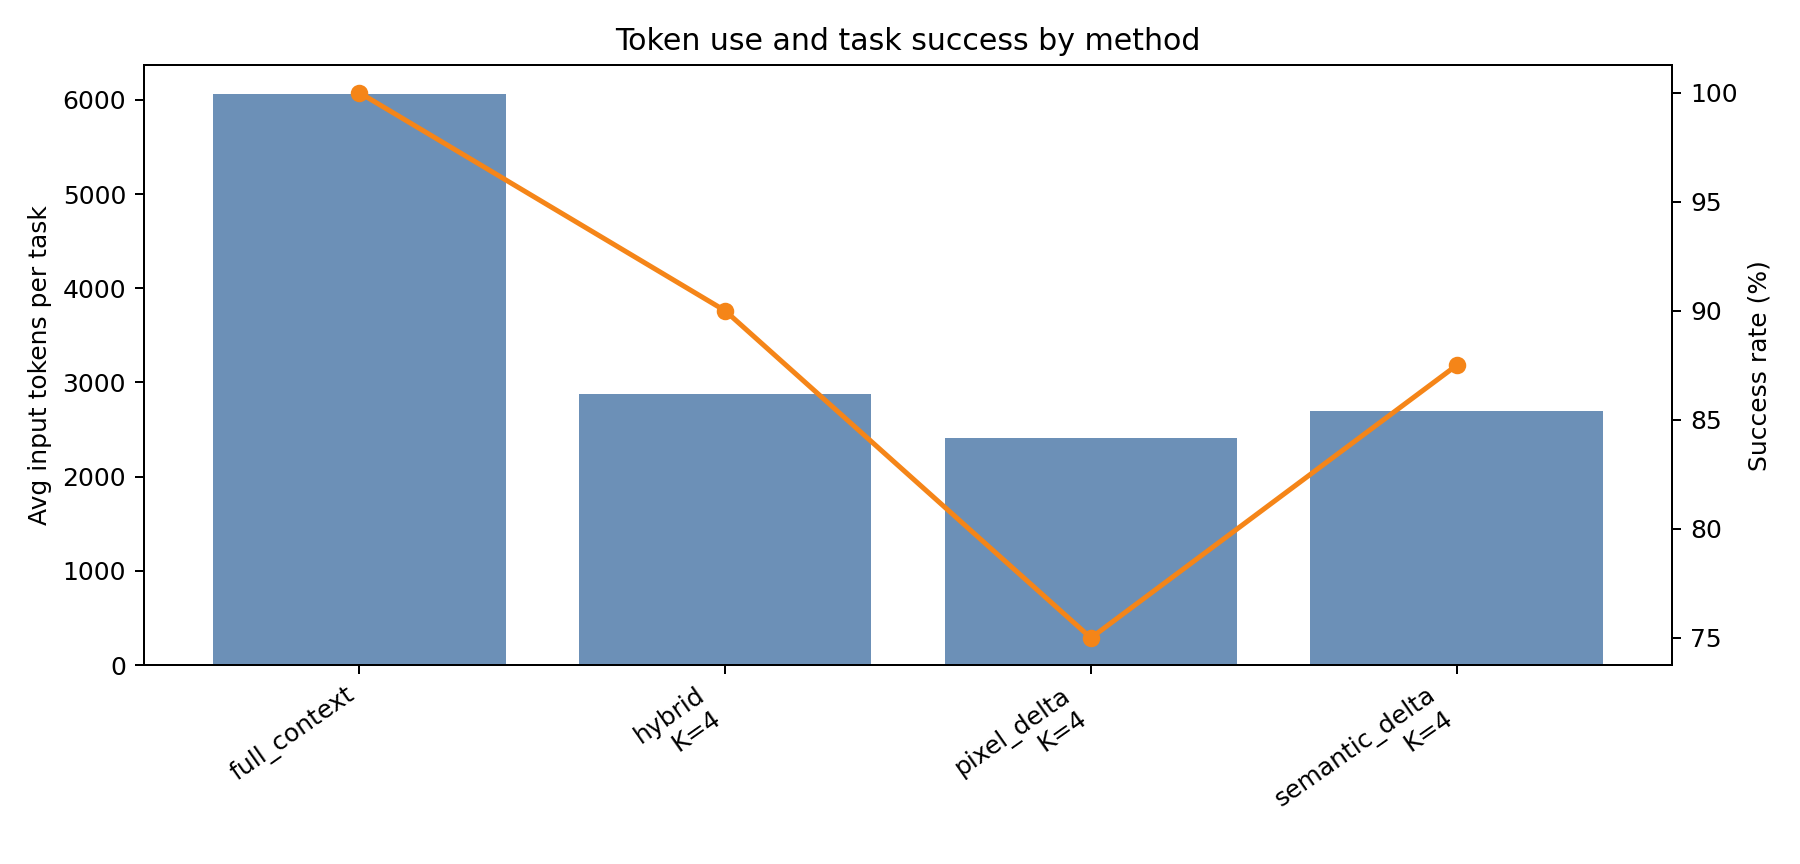
\includegraphics[width=0.95\linewidth]{figures/tokens_success_by_method.png}
\caption{Average input tokens and success rate by method.}
\label{fig:tokens-success}
\end{figure}

\begin{figure}[t]
\centering
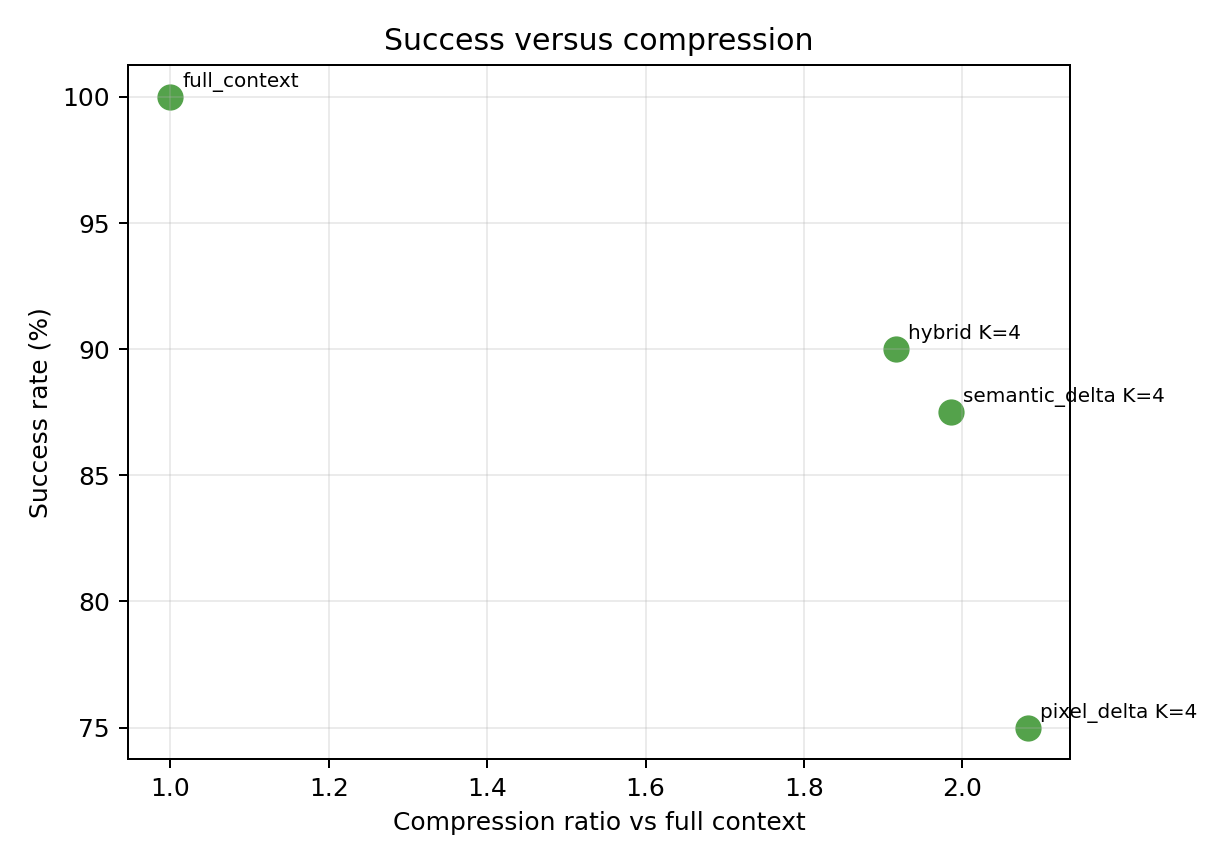
\includegraphics[width=0.72\linewidth]{figures/success_vs_compression_ratio.png}
\caption{Success versus compression ratio. The hybrid method occupies the intended region: large token reduction with moderate success loss.}
\label{fig:success-compression}
\end{figure}

\section{Ablations}

The repository includes scripts for keyframe interval, compression type, and history compression ablations. The keyframe interval ablation compares $K \in \{1,2,4,8,16\}$, while the compression ablation compares full context, pixel deltas, semantic deltas, and hybrid deltas. The history ablation compares no compression, summary, action-only history, and state-summary history. The main draft reports the default run; future workshop revisions should include the full ablation table after connecting real model calls.

\section{Failure Analysis}

The synthetic failure taxonomy tracks missing visual detail, bad delta reconstruction, wrong action prediction, stale keyframes, semantic parser errors, and task ambiguity. Pixel deltas achieve the strongest compression in the default run but lose more task success, because they do not expose enough semantic structure. Semantic deltas recover some success but can miss visual layout cues. Hybrid compression reduces both problems by preserving periodic visual anchors and explicit semantic changes.

\begin{figure}[t]
\centering
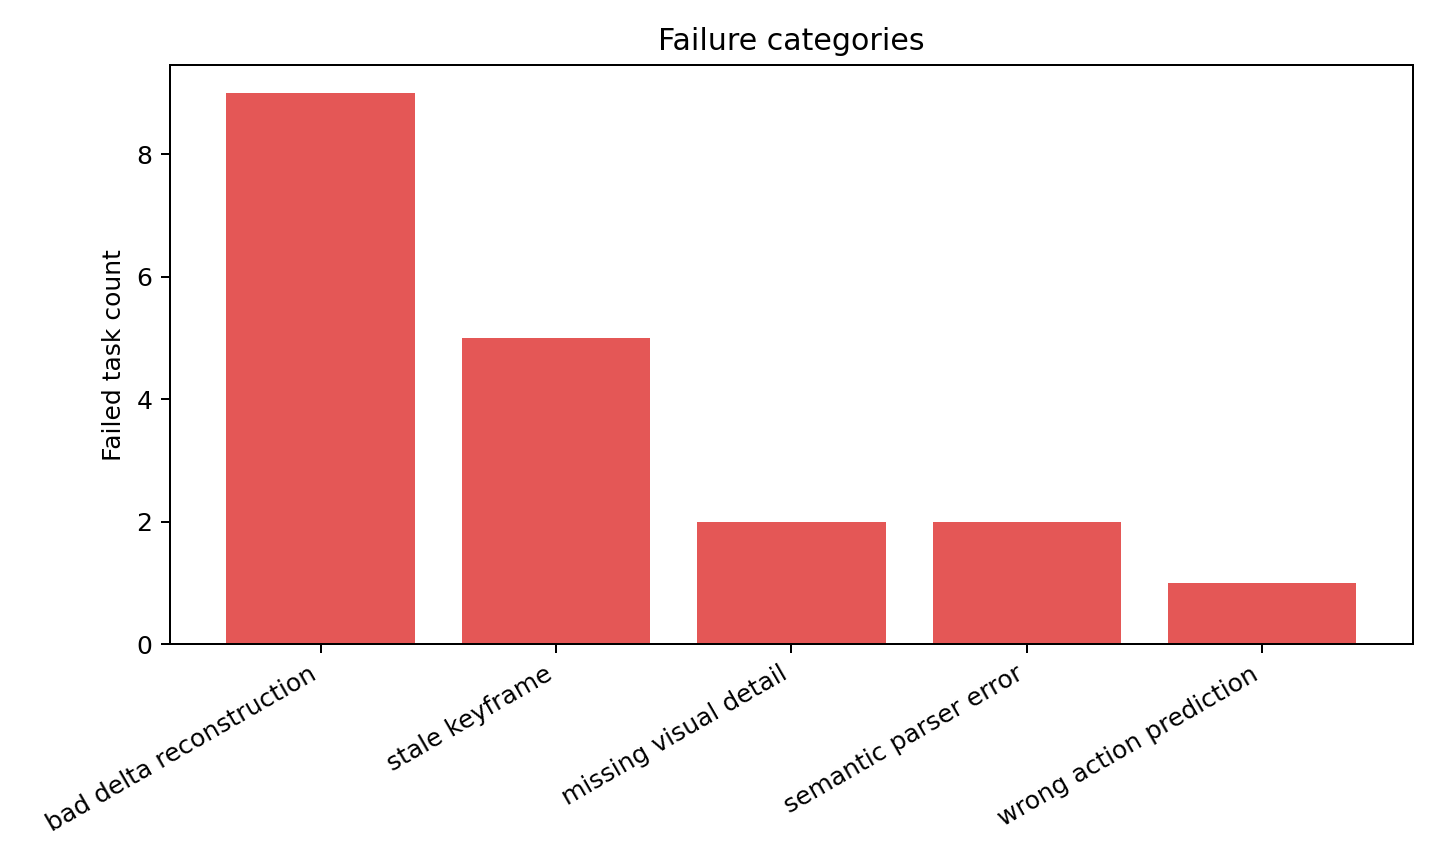
\includegraphics[width=0.78\linewidth]{figures/failure_categories.png}
\caption{Failure categories from the default synthetic benchmark.}
\label{fig:failures}
\end{figure}

\section{Limitations}

The present system is a research prototype. The default benchmark is synthetic and uses a deterministic simulated decision policy rather than real model calls. The DOM and accessibility parsers are intentionally simple. Pixel deltas are bounding-box-level hints rather than perceptual descriptions. The latency and cost estimates are modelled from token counts rather than measured from a hosted model. These limitations are acceptable for a workshop prototype but must be addressed before making strong benchmark claims.

\section{Conclusion}

GUI interaction trajectories are highly redundant. This paper frames computer-use agent context as a temporal stream and implements a practical keyframe plus delta encoding system. In a 40-task custom benchmark, hybrid GUI compression cuts input tokens by 52.5\% and reduces simulated latency while preserving 90.0\% success. The next step is to replace simulated decisions with real model calls and run the same compression interface on WebArena, VisualWebArena, and OSWorld subsets.

\bibliographystyle{plain}
\bibliography{references}

\end{document}
